\section{User Interface}\label{sec:design_ui}

In this section we will cover the development of the user interface (UI). First we will cover the requirements and the task that the UI is responsible for solving. Then we will discuss the demographics of our envisioned potential users, before finally covering the implementation. 

As a mean to derive requirements, we initially developed an information flow diagram of the UI. This outlined the usage of the system allowing us to consider the different use cases and user needs.

\subsection{Information Flow}

\begin{figure}[tbp]
\centering
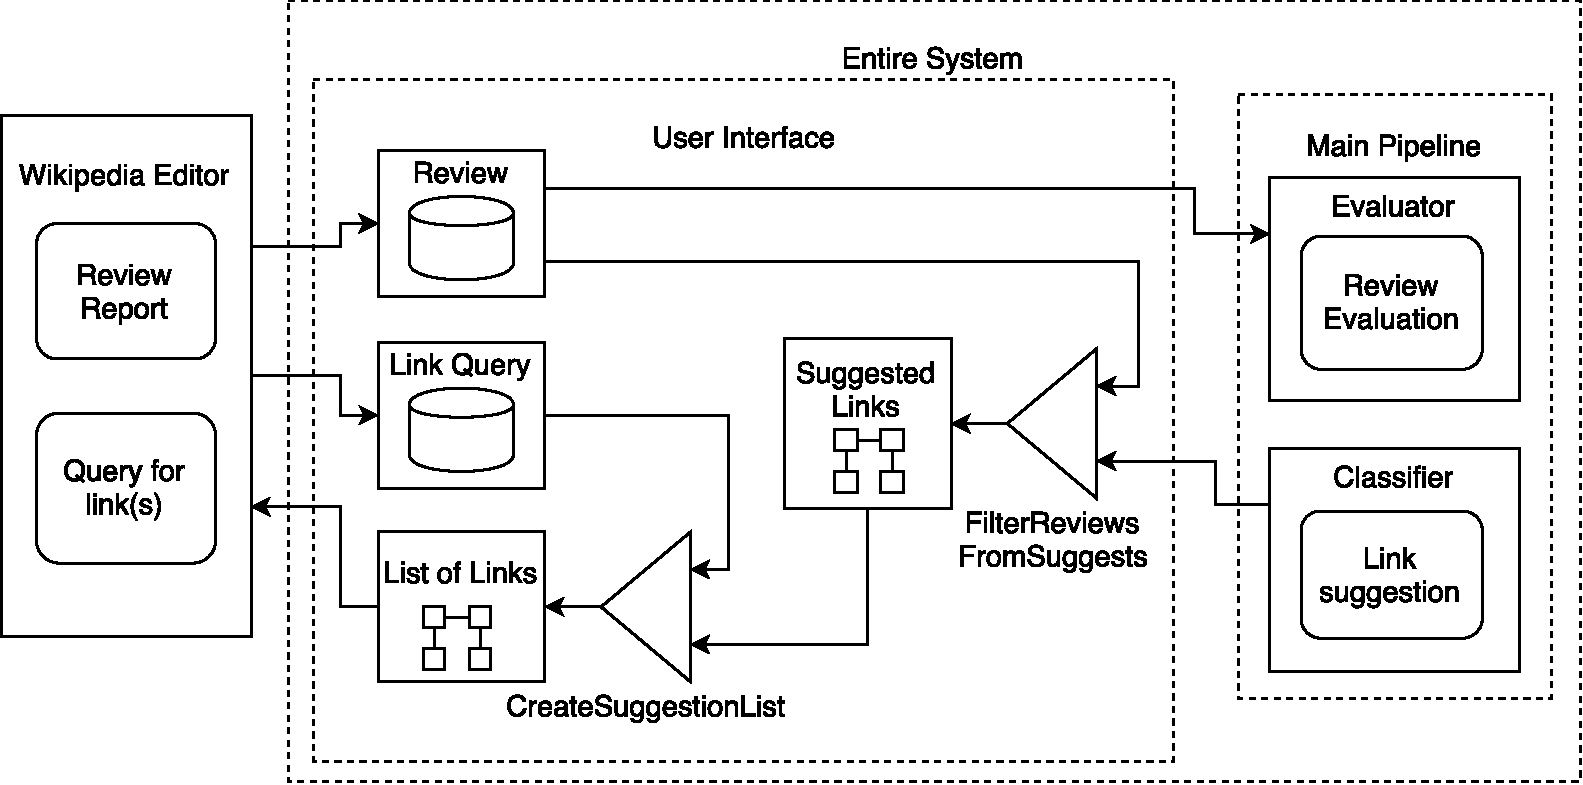
\includegraphics[width=0.95\textwidth]{wikiAPI.pdf}
\caption{Information flow diagram for user interface.}\label{fig:information_flow_UI}
\end{figure}	

In the diagram seen in \cref{fig:information_flow_UI}, which is in the WebML+ style~\cite{Casteleyn2009}, we have the two actors and the UI\@. One actor is the Wikipedia Editor and the other is the main pipeline. While the main pipeline could be modeled as a system with its own information flow, it is more beneficial for the requirement engineering process to simplify the main pipeline as an actor outside of the UI, since the requirements for the UI should not be affected by the inner workings of the main pipeline.

The Wikipedia Editor actor has two actions. First is the \enquote{Query for Link(s)} action, which prompts the UI for links to be evaluated. Secondly we have a \enquote{Review Report} action, where the actor informs the UI whether a previously suggested link was added to Wikipedia or not.

While other actions by the Wikipedia Editor actor could easily be conceived, we will argue that these two represent the primary actions, with the \enquote{Query for Link(s)} action being the essential one. By only including these two, we keep the initial requirement analysis focused on the core requirements, and leave further expansion for later iterations.


\subsection{Requirements}

From this diagram two functional requirements can be deducted. There is a requirement for retrieval of link suggestions and a requirement for the reporting of link reviews.

In the case of the retrieval of link suggestions the information flow is as follows:

\begin{enumerate}
	\item The classifier supplies the UI with link suggestions
	\item The reviewed links are filtered from the link suggestions
	\item A Wikipedia Editor queries the UI for links
	\item The query is used to create a list of links for the Editor
\end{enumerate}

For the case of reporting link reviews, where a user reports their evaluation of a suggested link, the information flow is as follows:

\begin{enumerate}
	\item The users submits a review of a suggested link
	\item The review is used for filtering link suggestions
	\item The review is also forwarded to the main pipeline for further evaluation
\end{enumerate}

The last step of forwarding the review to the main pipeline represents a future use of the reviews to re-train the classifier. This is not a current consideration in the main pipeline, but the UI is designed to support this type of feedback.

The requirements found in these two information flows are:

\begin{itemize}
	\item A user must be able to query the UI for link suggestions
	\item A user should be able to submit reviews of link suggestion
\end{itemize}

\subsection{User Demographic}

In order to design a solution for the requirements, we first consider the envisioned user demographic. The user is a Wikipedian, i.e. a person who edits Wikipedia articles. The Wikipedians we especially wish to engage are the so called coolfarmers, which is a term coined by~\cite{coolfarming}, to describe the top editors of Wikipedia. They cite~\cite{Priedhorsky:2007:CDR:1316624.1316663} with the findings that the editing of Wikipedia is a long tail distribution, and through an analysis of behavioral patterns identify the coolfarmers as the backbone of Wikipedia~\cite{coolfarming}. Furthermore~\cite{wiki_motivation} has found that \enquote{fun} and \enquote{ideology} are the two most important reasons why users edit Wikipedia, and~\cite{Yang20101377} extends on this by finding that internal self-concept-based motivation\footnote{motivation by feeling a personal achievement when sharing knowledge and being a self-motivated person} is the most important type of motivation for the Wikipedians.

We believe that the most effective way employ the results of the main pipeline, is to focus on delivering them to the coolfarmers and thereby combining the computational power of a classifier with their experience and motivation to make the actual edits.


\subsection{Web API}

Our choice of UI is a web API that allows users to access and review the information we can provide. What follows is a justification for this choice, as well as some specifics as to the implementation of the UI.

\subsubsection{Choosing API}
Since Wikipedians are often driven by self-motivation and ideology we believe that the most important function of the UI is to deliver the information effectively. We believe that this delivery should allow the community to get the best results into the articles of Wikipedia.

It can easily be argued that a website or a browser plug-in that focuses on a graphical representation of the results, will have a wider reach than an API that delivers the raw data. While such implementations could, if successful, provide the project a boost in popularity, there is a significant chance that the given implementation would not gain popularity.

However if we focus on making the results accessible, we can hope to benefit from the Wikipedia community, and possibly spark other projects of interface development. And even if this is not the case, we can proceed to build a graphical interface ourselves, upon the already working API.

\subsubsection{Implementation}

The API was developed as a RESTful~\cite{rest} API using HTTP methods. The REST architecture style was chosen due to its popularity and simplicity, two properties that fit well with out requirements and envisioned user demographic. We developed two endpoints which are described in \cref{rest_table}. The current implementation handles data in a JSON format, but this could easily be extended to multiple data formats.

\todo{add caption to table}
\begin{table}[]
\centering
\label{rest_table}
\begin{tabular}{@{}|p{0.10\textwidth}|p{0.30\textwidth}|p{0.30\textwidth}|p{0.30\textwidth}|@{}}
\toprule
HTTP Method & Description & Arguments & Example Result \\ \midrule
GET         & Returns a list of link suggestions that requires evaluation & An integer limit for the maximum returned links.
			& \mono{[\{"source":Jesus, "target":Gabriel\}, \{"source":Elephant, "target":Tiger\}]} \\ \midrule
POST        & Accepts a submission of a review & Requires source, target, and status to be defined. Status must have the value of either "good" or "bad". & Review Accepted \\ \bottomrule
\end{tabular}
\end{table}

\subsubsection{Security Concerns}

One thing that needs revision before the current implementation can be put to use, is security concerns. Since the POST method indirectly extends access to storage on the server, this could be the target of malicious usage. We have classified our security concerns into two catagories: technical and non-technical. The technical concerns deal with malicious use that seeks to exploit a technical flaw. Examples of these could be attempts of maxing out our storage or trying to inject code into our system. The non-technical types is by definition anything else, but examples could be the submission of bad reviews, maliciously or not.

While the technical concerns are important, these are not unique to our system and the use of a reliable framework would do much to prevent these. The non-technical concerns however are largely unique to our system, and as such the preventive measures requires more focus from our side. For the problem of bad reviews, the first step is to register that a review is bad. Our two primary ideas is to either monitor Wikipedia to check whether a review conteniously matches the state of the given article, or to consider if multiple reports on the same review agrees.

If we detect a review we consider bad the removal of it is a trivial task. However, in order to detect whether the review was malicious we would probably need to consider whether the same user gives repeated bad reviews. This is a non-trivial task. The direct way to solve this would be to require users to register in our system, but this would make the API less accessable. It would be worth exploring if we could detect malicious users solely through logs, but this is not guaranteed to give good results.